\chapter*{Task 1: Basic Probabilities and Visualizations (1)}
%\addcontentsline{tableofcontents}{chapter}{Task 1: Basic Probabilities and Visualizations (1)}

The parameter generator provided the following values:
\[
\xi_1=0,\qquad \xi_2=0.62.
\]

In this task, a voter must choose one of two possible answers: either ``for'' or ``against''. Before the vote
takes place, we do not know which answer will be selected, but the
probability model specified in the assignment allows us to describe
the uncertainty mathematically.

A Bernoulli random variable represents a single trial with two possible
outcomes, conventionally called success and failure (ref).

To describe the vote numerically, we define the random variable $X$ by
\[
X=
\begin{cases}
1, & \text{if the vote is for},\\
0, & \text{if the vote is against}.
\end{cases}
\]
This definition makes a vote in favour the ``success'' outcome and a
vote against the ``failure'' outcome. The numerical encoding is a
modelling choice; it does not change the voting situation itself.

By the definition of a Bernoulli distribution, its parameter $p$
is the probability of success, with $0\leq p\leq 1$. The task
specifies that the probability of voting ``for'' equals $\xi_2$.
Consequently,
\[
X\sim\text{B}(p),
\qquad p=\xi_2=0.62.
\]
It follows directly that
\[
P(X=1)=p=0.62.
\]
Since the only other possible outcome is $X=0$, its probability is
the complement of the probability of voting ``for'':
\[
\begin{aligned}
P(X=0)
&=1-P(X=1)\\
&=1-0.62\\
&=0.38.
\end{aligned}
\]
Thus, the probability model assigns probability $0.62$ to a vote
in favour and probability $0.38$ to a vote against.

\subsection*{Interpreting and visualizing the probabilities}

The probabilities can be expressed as percentages by multiplying
each probability by $100\%$. Therefore,
\[
P(\text{vote = ``for''})=0.62\cdot100\%=62\%
\]
and
\[
P(\text{vote = ``against''})=0.38\cdot100\%=38\%.
\]

These percentages describe the probabilities specified by the model.
They do not mean that a single vote is partly ``for'' and partly
``against'': the outcome of the individual trial is one or the other.
The percentages quantify the model's uncertainty before the outcome
is observed.

A bar chart is an appropriate visualization because there are two
discrete outcomes, each associated with a probability. Figure
\ref{fig:task1_vote} displays the probabilities, with the voting
outcomes on the horizontal axis and probability in percent on the
vertical axis. The vertical scale runs from $0\%$ to $100\%$.

\begin{figure}[h]
    \centering
    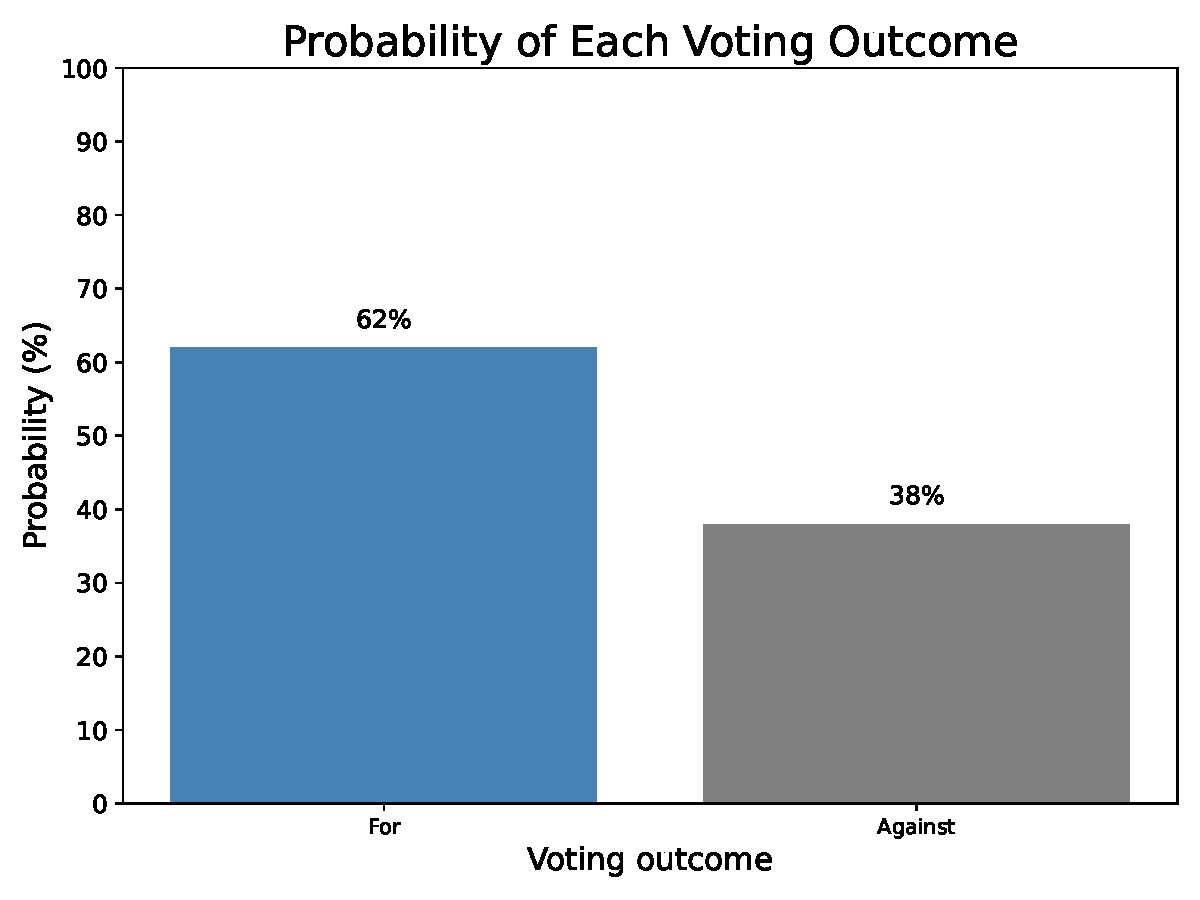
\includegraphics[width=0.7\textwidth]{pics/task1_bernoulli.pdf}
    \caption{Probability distribution for a single vote, using $\xi_2=0.62$ (code provided below)}
    \label{fig:task1_vote}
\end{figure}

Before accepting these values as a valid probability distribution,
we can verify the two basic requirements. First, neither probability
is negative:
\[
0\leq 0.38\leq 1,
\qquad
0\leq 0.62\leq 1.
\]
Second, because the two outcomes are mutually exclusive and
exhaust all possibilities for this vote, their probabilities must
sum to one. Indeed,
\[
P(X=0)+P(X=1)=0.38+0.62=1.
\]
Both requirements are satisfied. Hence, the calculated probabilities
form a valid distribution for the random variable $X$.

The figure is generated from these calculated values rather than
from simulated votes. This distinction matters: simulation would
produce random observed proportions, whereas the bars in Figure
\ref{fig:task1_vote} display the probabilities specified by the
model.

\subsection*{Can the expected value be calculated?}

The next question is whether the random outcome has an expectation.
To answer it, we must distinguish the original categorical answers
from the numerical random variable $X$ defined above. The words
``for'' and ``against'' do not, by themselves, have numerical values
whose average can be calculated. Our definition of $X$, however,
assigns the values $1$ and $0$ to these outcomes, so its expectation
is mathematically meaningful.

For a discrete random variable, the expectation is defined as the
sum of each possible value multiplied by its probability. When
the random variable has finitely many possible values, this sum
is finite and the expectation exists (ref). In this exercise, the definition gives
\[
E[X]=\sum_{x\in\{0,1\}}xP(X=x).
\]
Substituting the two possible values and their probabilities yields
\[
\begin{aligned}
E[X]
&=0\cdot P(X=0)+1\cdot P(X=1)\\
&=0\cdot0.38+1\cdot0.62\\
&=0+0.62\\
&=\boxed{0.62}.
\end{aligned}
\]

For completeness, the existence of the expectation can also be
verified using the sufficient condition $E[|X|]<\infty$. Since
$X$ can take only the values $0$ and $1$, we obtain
\[
\begin{aligned}
E[|X|]
&=|0|P(X=0)+|1|P(X=1)\\
&=0\cdot0.38+1\cdot0.62\\
&=0.62<\infty.
\end{aligned}
\]
Therefore, $E[|X|]$ is finite, which establishes that the expectation
of $X$ exists and is finite.

The result has a straightforward interpretation. The random variable
$X$ equals one when the voter votes ``for'' and zero otherwise.
Consequently, its expected value equals the probability of voting
``for'':
\[
E[X]=P(X=1)=0.62.
\]

In repeated comparable voting situations, the expected value describes
the long-run average of the numerical indicator, not the outcome of
the individual vote. It does not imply that a particular vote will
equal $0.62$; an observed value of $X$ must be either zero or one.

The numerical encoding should also be kept in mind. If we had instead
defined $X=1$ for ``against'' and $X=0$ for ``for'', the expectation
would have been $0.38$. The probabilities of the actual voting
outcomes would remain unchanged. Thus, an expectation for categorical
outcomes depends on the numerical representation chosen, and that
representation must be stated explicitly.

\noindent

\lstinputlisting[language=Python]{task1_plot.py}

\chapter*{Task 2: Basic Probabilities and Visualizations (2)}
%\addcontentsline{tableofcontents}{chapter}{Task 2: Basic Probabilities and Visualizations (2)}














































\section{Tools}

MiKTeX: \url{https://miktex.org/download}
TeXLive: \url{http://tug.org/texlive/}
 (or alternative LaTeX-systems).
 
 A good editor is essential. Sometimes combined editors and compilers (e.g. TeXShop) can be really productive. Make sure you learn the use of synchronized navigation then.

\begin{figure}[h]
\centering
\includegraphics[width=8cm]{pics/spiral.pdf}
\caption{A spiral... smooth vector-based with a clean parametrisation! \\ Nothing to do with \textcite{Gage:18}}\label{fig:spiral}
\end{figure}
\FloatBarrier

\section{Tables}

\begin{table}[H]
\small
\centering
\begin{tabular}{p{5cm}|l|p{3cm}}
`` Industrial era '' &  ``Jobs '' & `` Wanted: Upgrade''' \\ \hline
Parts exchanger & Fitter & mecatronics specialist \\
eShop & reseller & `` Client-suggester'' \\
`` Coding-guru''' & Softwaredesign & Whole-life designer \\
JA! Gut \& Günstig & brand-names & `` Life-Style Feeling'' \\
Internetbanking & Bank clerk & Customer adviser \\
Robots & Specialist & Machine supervisor \\
Bush & Gardener & Nature-sculptor \\
Painting & Painter & Interior Design \\
 &  & \\
\end{tabular}
\caption[Downgrade and upgrade of job denominations]{Downgrade and Upgrade of job denominations \\ \ \ \ \textcite{DueckKo:2016}}
\label{tab:Downgrade and Upgrade of job denominations}
\end{table} 

\section{Listes}

\begin{itemize}
 \itemsep0pt
 \item one
 \item twoi
 \item threei
\end{itemize}

\begin{enumerate}
 \itemsep0pt
 \item first
 \item second
 \item third
\end{enumerate}


\section{Formulæ}

A formula can be written inline, e.g. as $ \frac{d}{dx}\mbox{arctg}(x) = \frac{1}{1+x^2}$ or, in centered math:

\begin{equation}  \frac{d}{dx}\mbox{arctg}(x) = \frac{1}{1+x^2} \label{arctanderivative}\end{equation}

Notice that formulæ that are centered start bigger (technically, they start in \verb+\displaystyle+) than they start inline (technically, they start in \verb+\textstyle+ all subsequents reductions, e.g. an exponent, goes to \verb+\scriptstyle+ then \verb+\scriptscriptstyle+). Indeed a best effort is made so that inline formulæ do not change the line height which would bother the eye of a reader.

Formulæ can be given a number and a label. Numbering happens automatically with \verb+\begin{equation}+ and \verb+\end{equation}+ and can be avoided if enclosing the formula between \verb+\[+ and \verb+\]+. If using the \verb+\label+ macro inside, you can refer automatically to this equation using \verb+\ref{label}+. E.g. Thanks to equation~\ref{arctanderivative} one dare say that:

\begin{equation} \int_0^t \frac{1}{1+x^2} dx = \mbox{arctan}(t) \end{equation}


\section{Tools and Code}

Many users of this template will want to include some code.

The simplest way to do so is to use the \verb+\verb+ macro which is followed by a sign, then some code, then the sign again to close. This is the inline version which works as in: 


\begin{verbatim}
As we could calculate with \textcite{Wolfram_Alpha} using 
\verb_integrate 1 / pi e ^ (t/pi) from zero to infinity_.
\end{verbatim}

which yields: 

As we could calculate with \textcite{Wolfram_Alpha} using \verb_integrate 1 / pi e ^ (t/pi)_ from zero to infinity.


The multiline version of this is called \verb+\begin{verbatim}+ and finishes with \verb+\end{verbatim}+.


\section{Citation examples}

Monography \parencite[p.~22]{con:infra} 

Collection \parencite{sammelband} 

Article \parencite{article1}
